%% LyX 2.5.1 created this file.  For more info, see https://www.lyx.org/.
%% Do not edit unless you really know what you are doing.
\documentclass[brazil]{article}
\usepackage[T1]{fontenc}
\usepackage[utf8]{luainputenc}
\usepackage{babel}
\usepackage{graphicx}
\usepackage[]
 {hyperref}

\makeatletter

%%%%%%%%%%%%%%%%%%%%%%%%%%%%%% LyX specific LaTeX commands.

%% Because html converters don't know tabularnewline
\providecommand{\tabularnewline}{\\}

\makeatother

\begin{document}

\section{Moeda}

\subsection{Teoria Estatal da Moeda}

O que pretendo apresentar é uma breve discussão que abrange principalmente as 15 páginas entre as seções “11.2 Duas teorias do dinheiro” e “11.4 Espaço monetário, uma ilustração” do ``Classical Econophysics''\cite{cockshott2012classical}, com o objetivo de ilustrar a Teoria Estatal da Moeda (STM em inglês).

Nessa teoria, o Estado decide o que conta como dinheiro, estipulando o que aceitará como pagamento por obrigações. Em outras palavras, o Estado pode criar um determinado tipo de moeda exigindo que os cidadãos paguem seus impostos nessa moeda. A necessidade de prevenir a falsificação pode favorecer a ideia de criar moeda a partir de uma substância específica, mas não há uma conexão inerente entre o valor do dinheiro enquanto dinheiro e seu valor enquanto metal. 

Acredito ser interessante apresentar esta teoria pois ela está na base da Teoria Monetária Moderna (MMT em inglês) que tem ganhado a atenção de economistas heterodoxos e mesmo em marxistas como uma alternativa para explicar a dinâmica da moeda na sociedade moderna.

Nesta teoria podemos dizer que o dinheiro tem três funções:
\begin{itemize}
\item \textbf{Meio de troca}: O dinheiro é usado como intermediário na troca de outras mercadorias que são de interesse primordial para os comerciantes.
\item \textbf{Unidade de conta}: Preços, dívidas, etc., são denominados na unidade monetária.
\item \textbf{Reserva de valor}: As pessoas podem armazenar sua riqueza na forma de dinheiro.
\end{itemize}
Nessa concepção de dinheiro, sua função como unidade de conta é vista como primordial. A unidade monetária denomina a dívida do cidadão para com o Estado.

Há algumas evidência históricas que são costumeiramente relembradas para defender a TEM. Primeiro há um contra-exemplo para a ideia de que moedas surgiram apenas para fornecerem um peso padrão para metais preciosos, como uma evolução natural da prática de usar uma mercadoria intermediária como unidade de conta (neste caso, um metal precioso). Na Mesopotâmia antiga transações comerciais foram registradas em unidades de Shekels, que possuiam um equivalente em cevada ou prata. Mas as transações não eram feitas em prata. Além disso, as primeiras moedas estavam longe de terem um peso padronizado.

Mas o que acredito ser mais interessante de ser discutido diz respeito à relação coercitiva entre o estado e a população mediada pelo dinheiro. O livro apresenta a seguinte citação de Forstater:
\begin{quote}
Se a base de subsistência fosse capaz de sustentar toda a população, os súditos coloniais não seriam obrigados a oferecer sua força de trabalho para venda. Os governos coloniais, portanto, necessitavam de meios alternativos para obrigar a população a trabalhar por um salário. O registro histórico demonstra claramente que um método muito importante para alcançar esse objetivo era a imposição de um imposto e a exigência de que a obrigação tributária fosse paga em moeda colonial. Esse método tinha a vantagem não só de forçar as pessoas a trabalhar por um salário, mas também de criar valor para a moeda colonial e monetizar a colônia. Além disso, esse método podia ser usado para forçar a população a produzir produtos agrícolas para venda. O que a população tinha que fazer para obter a moeda ficava inteiramente a critério do governo colonial, já que este era a única fonte da moeda colonial.
\end{quote}
Em seguida, passamos a discutir os registros e relações monetárias. Cabe observar que, quando o Estado muda de tributar bens para tributar dinheiro, ele passa de uma apropriação direta (quando o camponês tinha o dever de fornecer tempo de trabalho ou colheita ao Estado) para uma indireta (nosso sistema atual), mediada pelo dinheiro. Além disso, para operar um sistema monetário baseado em contas, algo mais abstrato onde o dinheiro é digital por exemplo, é necessária uma classe instruída, visto que esse sistema exige habilidades matemáticas e tecnologia mais avançada; também exige que um sistema seguro e confiável de escrita e armazenamento tenha sido desenvolvido.

Em um sistema baseado em moedas físicas, como metais preciosos, esses requisitos são menores. Por exemplo, a quantia de dinheiro que cada indivíduo possui é obtida simplesmente verificando o número de moedas que ele detém. Ou seja, a presença física das moedas em uma bolsa representa um número; a posse dessa bolsa por um indivíduo define a posse desse dinheiro. Em outras palavras, quando passamos de um sistema baseado em contas para um baseado na cunhagem de moedas, temos um processo de descentralização; este último é flexível e de baixa tecnologia. Uma limitação evidente é que não é possível ter um número negativo de moedas.

Mas meu principal objetivo aqui é ilustrar o mecanismo pelo qual uma economia monetizada por uma potência colonizadora é explorada. O exemplo dado apresenta algumas semelhanças com a Nigéria em 1905 e o Império Britânico.

\textbf{Etapa 0}: Começamos com um estado inicial sem dinheiro ou obrigações.
\begin{center}
\begin{tabular}{|c|c|c|}
\hline 
Agente & Dinheiro & Obrigações com Imposto\tabularnewline
\hline 
\hline 
Estado & 0 & 0\tabularnewline
\hline 
Ana & 0 & 0\tabularnewline
\hline 
Tiago & 0 & 0\tabularnewline
\hline 
Felipe & 0 & 0\tabularnewline
\hline 
Total & 0 & 0\tabularnewline
\hline 
\end{tabular}
\par\end{center}

\textbf{Etapa 1}: O Estado emite a moeda.
\begin{center}
\begin{tabular}{|c|c|c|}
\hline 
Agente & Dinheiro & Obrigações com Imposto\tabularnewline
\hline 
\hline 
Estado & 9 & 0\tabularnewline
\hline 
Ana & 0 & 0\tabularnewline
\hline 
Tiago & 0 & 0\tabularnewline
\hline 
Felipe & 0 & 0\tabularnewline
\hline 
Total & 9 & 0\tabularnewline
\hline 
\end{tabular}
\par\end{center}

\textbf{Etapas 2 e 3:}

2. O Estado emprega Felipe no exército e lhe paga 7 moedas;

3. O Estado anuncia uma obrigação tributária de 2 moedas para todos.
\begin{center}
\begin{tabular}{|c|c|c|}
\hline 
Agente & Dinheiro & Obrigações com Imposto\tabularnewline
\hline 
\hline 
Estado & 2 & 6\tabularnewline
\hline 
Ana & 0 & -2\tabularnewline
\hline 
Tiago & 0 & -2\tabularnewline
\hline 
Felipe & 7 & -2\tabularnewline
\hline 
Total & 9 & 0\tabularnewline
\hline 
\end{tabular}
\par\end{center}

\textbf{Passo 4:} Como Ana e Tiago precisam pagar o imposto na nova moeda para não serem punidos, eles vendem comida para Felipe em troca de moedas.
\begin{center}
\begin{tabular}{|c|c|c|}
\hline 
Agente & Dinheiro & Obrigações com Imposto\tabularnewline
\hline 
\hline 
Estado & 2 & 6\tabularnewline
\hline 
Ana & 3 & -2\tabularnewline
\hline 
Tiago & 2 & -2\tabularnewline
\hline 
Felipe & 2 & -2\tabularnewline
\hline 
Total & 9 & 0\tabularnewline
\hline 
\end{tabular}
\par\end{center}

\textbf{Etapa 5}: Chega o dia da cobrança de impostos e os impostos são pagos.
\begin{center}
\begin{tabular}{|c|c|c|}
\hline 
Agente & Dinheiro & Obrigações com Imposto\tabularnewline
\hline 
\hline 
Estado & 8 & 0\tabularnewline
\hline 
Ana & 1 & 0\tabularnewline
\hline 
Tiago & 0 & 0\tabularnewline
\hline 
Felipe & 7 & 0\tabularnewline
\hline 
Total & 9 & 0\tabularnewline
\hline 
\end{tabular}
\par\end{center}

Felipe gastou todo o seu dinheiro e precisa ser contratado novamente. Tiago vendeu parte da sua produção apenas para cobrir a dívida. Ana guardou uma moeda e agora está em condições de atuar como comerciante; embora tenha trocado comida útil por uma moeda sem utilidade “real”, ela obteve um avanço social: agora possui uma moeda do rei e, portanto, participa indiretamente do poder e da autoridade real. Com essa moeda, ela pode comandar o trabalho de seus pares. À primeira vista, a compra pode parecer um símbolo de reciprocidade e de uma troca livre e voluntária, mas por trás dela reside um sistema de coerção e o medo da cobrança de impostos.

Finalmente, para concluir a discussão, em uma economia monetária, o Estado tem duas maneiras de acessar o trabalho da população. Ele pode cobrar um imposto em dinheiro e então gastar esse dinheiro na compra de mão de obra ou bens, ou pode simplesmente criar novo dinheiro. Os dois processos são interdependentes. Se não houver dinheiro inicial, é impossível cobrar um imposto; da mesma forma, se não houver imposto, o dinheiro não terá valor e o Estado não poderá apropriar-se de recursos reais com essa moeda.

Numa economia “natural”, a apropriação de recursos pelo Estado é direta e limitada pela sua capacidade política de coerção. Com a invenção do dinheiro, a apropriação dividiu-se em duas: uma apropriação simbólica de moedas através da tributação e uma apropriação real através da compra de tempo de trabalho e bens mediada pelo dinheiro. Desta forma, a apropriação real aparenta ser algo voluntário, enquanto o aspecto coercitivo do processo ocorre inteiramente no âmbito simbólico.

\subsection{Por um Econofisico}

Quero apresentar o artigo ``Economia Monetária sob uma Perspectiva Econofísica''\cite{Yakovenko2016}, escrito por Victor M. Yakovenko, onde, como ele mesmo afirma: ``o estilo deste artigo é bastante informal, e o foco principal está na fundamentação conceitual, em vez de detalhes técnicos de modelos matemáticos e dados empíricos''. Porém o código responsável por gerar as figuras pode ser encontrado no \href{https://github.com/jdansb/Econophysics/blob/main/files/monetary.ipynb}{meu GitHub}.

Dado que seu modelo possui importância indiscutível para estabelecer a desigualdade na distribuição de riqueza como um dos principais objetos de estudo da econofísica, acredito ser interessante abordar essa discussão conceitual sobre o aspecto monetário em seus modelos. Para começar, gostaria de destacar o resultado do modelo de Yakovenko:
\begin{quote}
\ldots existem poucos agentes ricos com saldos monetários elevados e muitos agentes pobres com saldos baixos, de modo que a distribuição é altamente desigual, embora os agentes sejam estatisticamente idênticos. Esta é uma conclusão chocante para as ciências sociais, onde a desigualdade é geralmente atribuída a diferenças intrínsecas entre os agentes. Há uma crítica de que muitos economistas não estão totalmente familiarizados com o conceito de equilíbrio estatístico, mas apenas com o de equilíbrio mecânico.
\end{quote}
Para prosseguir, precisamos começar com a definição de dinheiro: dinheiro é, portanto, apenas uma contabilidade digital, um token digital, ou seja, pode ser expresso como um número. Além disso, por sua própria natureza, o dinheiro deve necessariamente ser conservado, portanto, isso não é um artefato peculiar, mas um princípio contábil fundamental sobre o qual se baseia a funcionalidade do dinheiro. Isto é, os agentes envolvidos não podem produzir ou destruir dinheiro\footnote{Acredito a teoria monetária adotada pelo Yakovenko se aproximo a do Cockshott apresentada em ``Classical Econophsyics'' (livro do qual ele é co-autor) como Teoria Estatal da Moeda, conforme discutido anteriormente.}.

Isso fica explícito quando listamos as três propriedades do dinheiro: meio de troca, medida de valor e reserva de valor, que só fazem sentido se o dinheiro for conservado. Essas propriedades seriam perdidas se os agentes pudessem produzir dinheiro por conta própria.

\subsubsection{Criação de dinheiro}

Como o dinheiro pode surgir em um sistema onde os agentes não podem produzi-lo? Suponha que temos um sistema onde todos os agentes começam com 0 de dinheiro, mas quando um agente presta um serviço a outro, os saldos de ambos os agentes mudam de forma conservativa, ou seja, podemos simplesmente registrar que um agente agora tem um saldo negativo por ter ``pago'' e outro agente tem um saldo positivo por ter " recebido" ; é apenas uma questão de contabilidade. Contudo, o que acontece neste sistema se não houver limite inferior para saldos negativos? Poderia eu usufruir indefinidamente dos serviços de outros? Nesse sentido, é necessário impor um limite mínimo, de modo que, assim que um agente atinja esse saldo, ele não possa receber serviços sem fornecê-los.

Neste ponto, podemos simplificar o dinheiro deslocando todos os saldos de forma que o limite negativo seja agora zero. Isso equivale a dar inicialmente a cada agente uma quantia inicial de dinheiro igual em magnitude ao limite mínimo anterior. Assim, o saldo mínimo agora é zero, e o saldo inicial (ou agora, o dinheiro inicial) é uma quantia maior que zero. Como o dinheiro agora é positivo, poderíamos até usar objetos físicos como símbolos de dinheiro. Yakovenko cita a Teoria Monetária Moderna (MMT) como referência para discutir como o dinheiro é criado em escala nacional.

O que considero mais interessante são duas coisas. Primeiro, como já mencionado, a condição inicial dos saldos monetários entre os agentes, mesmo que sejam estatisticamente idênticos, não leva a uma distribuição igualitária de dinheiro. Segundo, citando Yakovenko:
\begin{quote}
A escola econômica do laissez-faire argumenta que, se todas as restrições e regulamentações forem removidas, a economia atingirá um equilíbrio natural e deverá permanecer assim. No entanto, esse argumento é enganoso, uma vez que o equilíbrio não pode ser alcançado sem a imposição de condições de contorno, ou seja, regulamentações.
\end{quote}
Para ilustrar a discussão, podemos trabalhar com um exemplo de código simples. Primeiro, vamos construir um modelo onde temos N agentes com 10 moedas cada. A cada passo, selecionamos aleatoriamente 2 agentes e transferimos uma moeda de um agente para o outro. O resultado em três instantes de tempo diferentes pode ser visto abaixo.

O que podemos observar é que este sistema sem restrições não atinge o equilíbrio. Conforme o tempo avança, a curva no histograma torna-se cada vez mais plana, nunca atingindo um verdadeiro equilíbrio, visto que é sempre possível para um agente aumentar sua dívida para um valor infinito.
\begin{center}
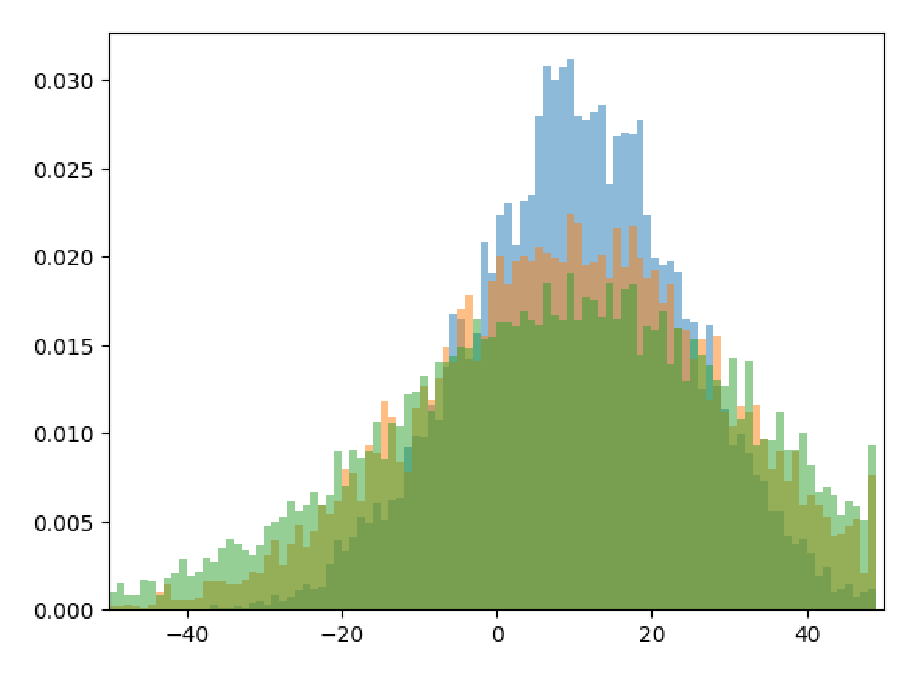
\includegraphics[scale=0.6]{colado1}
\par\end{center}

A seguir, realizamos uma simulação semelhante, mas agora definimos um limite inferior de 0. Ou seja, um agente não pode contrair dívidas. Se a riqueza de um determinado agente for 0, ele só poderá ganhar moedas, não podendo doá-las. Dois resultados podem ser observados aqui:

O sistema atinge o equilíbrio: podemos ver que o histograma em 3 instantes de tempo diferentes é qualitativamente o mesmo.

Embora as condições iniciais e as regras de troca sejam idênticas, a distribuição final de riqueza é altamente desigual.
\begin{center}
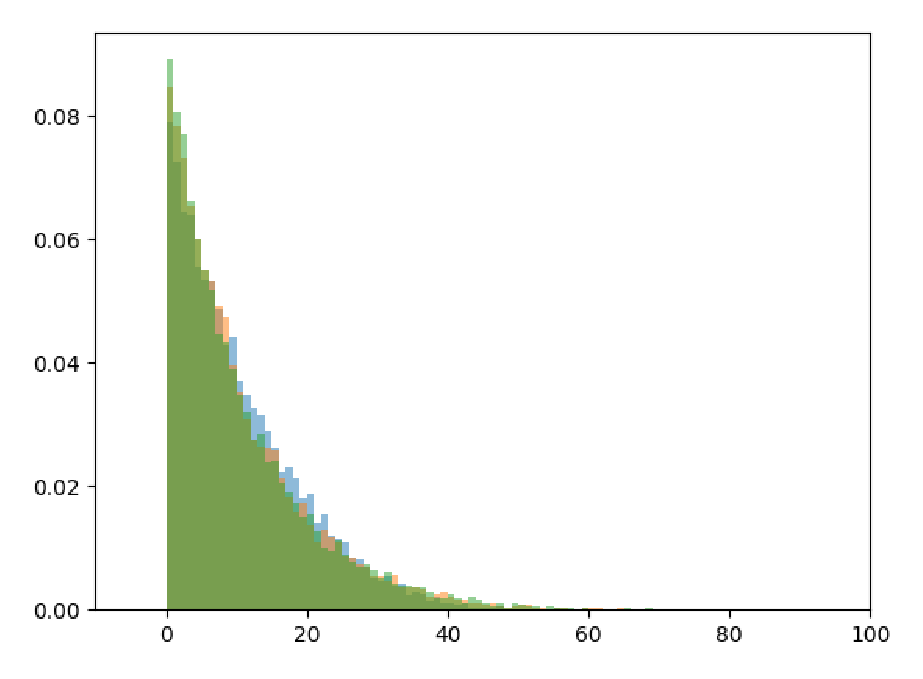
\includegraphics[scale=0.6]{colado2}
\par\end{center}

Invertendo nossa discussão, podemos ver que, se movermos o limite mínimo de 0 para -10 e, equivalentemente, a riqueza inicial for também 10 unidades menor do que no caso anterior, ou seja, agora cada agente começa com 0 moedas, podemos notar que o resultado é análogo ao caso anterior, apenas deslocado 10 unidades para a esquerda.
\begin{center}
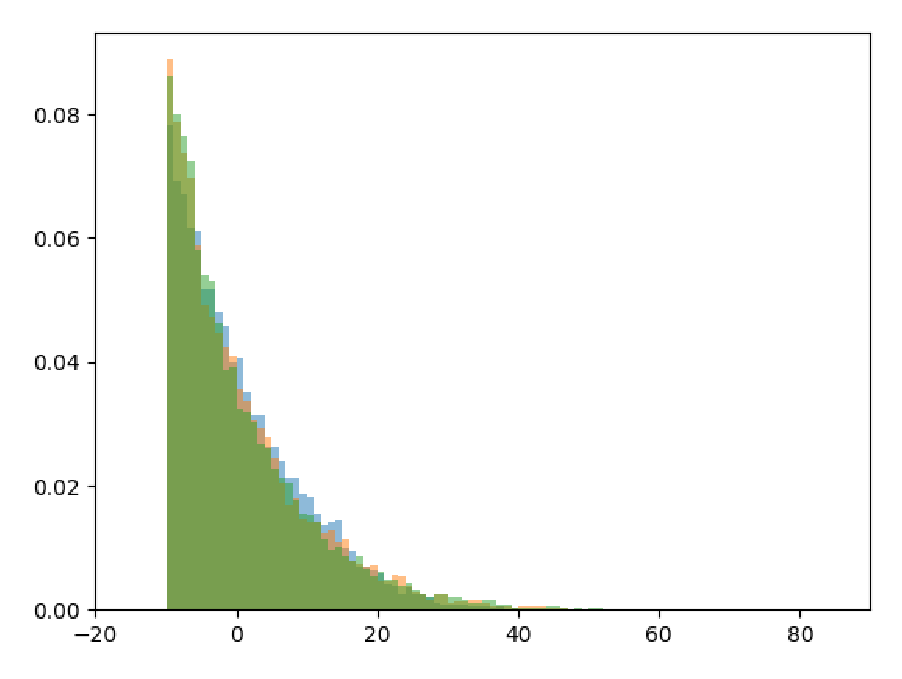
\includegraphics[scale=0.6]{colado3}
\par\end{center}

\subsubsection{As 12 falácias}

Na sequência, Yakovenko se propõe a discutir 12 falácias. São elas:

\textbf{Falácia 1}: O dinheiro cresce como resultado do investimento.

Afirma-se que, ao comprar US\$ 100 em ouro e vendê-lo anos depois por US\$ 200, a quantidade de dinheiro aumentou. Para avançar na discussão, precisamos distinguir entre o que o autor chama de duas camadas: uma camada física na sociedade, onde todas as coisas com existência física estão localizadas, e uma camada monetária, ou seja, relacionada ao dinheiro, uma camada informacional. As duas camadas estão acopladas e relacionadas, mas não são exatamente a mesma coisa. Neste exemplo, temos uma transação de ouro na camada física e uma transação monetária na camada informacional.

Neste caso, é necessário considerar todos os agentes envolvidos. De uma perspectiva individual, parece que o dinheiro aumentou, mas isso ocorre porque estamos analisando um único indivíduo. Nada neste exemplo implica necessariamente que o dinheiro deixa de ser conservado quando observamos o sistema como um todo. Mesmo que eu dê US\$ 100 a um agente em troca de ouro e, em seguida, dê esse ouro a outro agente em troca de US\$ 200 --- mesmo que esses agentes nunca interajam entre si, no caso mais extremo, isso implica apenas que já existiam US\$ 300 no sistema desde o início. Outro exemplo envolvendo investimento de fundos de pensão é discutido no artigo, bem como a seguinte leitura é recomendada: H. S. Dent, The Great Boom Ahead (Hyperion, Nova York, 1993).

\textbf{Falácia 2}: O dinheiro cresce como resultado da produção: Se o dinheiro é uma forma de medir a riqueza, e se a riqueza coletiva aumenta ao longo do tempo como resultado da produção, então o dinheiro também deveria aumentar.

No entanto, um aumento na produção, a expansão da camada física, não se traduz imediatamente na expansão da camada monetária. São coisas diferentes e seguem regras diferentes. Esse tipo de argumento é geralmente apresentado pela escola monetarista.

\textbf{Falácia 3}: A terceira falácia diz respeito a modelos econômicos sem dinheiro.

A maioria das crises econômicas recentes ocorre na camada monetária, não na física. Portanto, se tentarmos eliminar o dinheiro do modelo (assumindo um funcionamento ideal) não conseguiremos explicar as crises econômicas. Por outro lado, podemos reduzir o modelo à transferência de dinheiro entre agentes (abstraindo-nos das questões de produção) e ainda obter resultados interessantes. Essa é, por exemplo, a abordagem adotada em ``A Arquitetura Social do Capitalismo'' (Ian Wright)\cite{Wright_2005}.

Dinheiro e bens físicos pertencem a diferentes camadas da economia, mas geralmente são combinados em uma única variável chamada ``riqueza'', definida como $w_{i}=m_{i}+\sum_{j}p_{j}v_{ji}$, onde a riqueza do agente $i$ é dada em parte pela riqueza monetária ($m_{i}$) e em parte pelos produtos que ele possui, sendo o preço ($p_{j}$) um coeficiente de conversão que transforma unidades físicas, o volume ($v_{ji}$) do produto ($j$) detido pelo agente ($i$) --- em unidades monetárias.

Como combina conceitos de duas camadas diferentes, a riqueza se comporta de maneira distinta do dinheiro. Por exemplo, a riqueza pode crescer com a produtividade.

\textbf{Falácia 4}: Uma vez feita a distinção entre dinheiro e riqueza, uma crítica válida da econofísica pode ser direcionada a modelos que tentam interpretar a transferência e a conservação não de dinheiro, mas de riqueza. Embora matematicamente equivalentes, existe uma diferença conceitual.

Chegamos agora ao que provavelmente é um dos tópicos mais relevantes: a criação de dinheiro pelo Estado. Quando pensamos se o dinheiro é conservado (ou não), este é um dos principais pontos a serem levantados, afinal, o Estado tem a capacidade (que de fato exerce) de produzir dinheiro. É, portanto, natural perguntar como conciliar essa capacidade estatal com um modelo conservativo de dinheiro. Nesse sentido, Yakovenko define o sistema econômico como o conjunto de agentes privados, com o Estado considerado externo ao sistema. Nesse caso, o sistema é conservativo, mesmo que a quantidade total não seja mantida devido ao fluxo de entrada e saída de dinheiro proveniente das interações entre o sistema e os componentes externos. Em outras palavras, ao construir um modelo de um sistema econômico, o Estado é considerado externo e, sob essa condição, o dinheiro é conservado.

E quais são as motivações ou necessidades do Estado para injetar dinheiro no sistema? Uma razão entre muitas é o crescimento populacional. Se a população aumenta, mas a quantidade de dinheiro não, então o dinheiro per capita diminuirá, o que significa que o poder de compra de uma determinada quantia de dinheiro aumenta. Essa consequente queda nos preços é chamada de deflação, e assim que um agente percebe esse fenômeno, ele pode se sentir incentivado a reter dinheiro, já que poderá comprar mais bens no futuro, retirando, assim, mais dinheiro de circulação e acentuando a deflação. Pode-se, portanto, argumentar que o Estado deveria aumentar a quantidade de dinheiro pelo menos proporcionalmente com a população. Até mesmo a escola monetarista propôs uma regra monetária de injeção constante de dinheiro de acordo com um cronograma regular, argumentando que uma inflação moderada estimula a economia.

Se seguirmos o conceito de que o dinheiro deve ser ganho através do trabalho, a melhor maneira de o Estado injetar novos recursos é financiando projetos de infraestrutura pública que beneficiem a sociedade como um todo. Parte do financiamento desses projetos também pode ser coberta por impostos arrecadados pelo Estado; a proporção entre ambas as fontes é uma questão técnica e prática, não um dogma como o de um “orçamento governamental equilibrado”. Um exemplo prático desse tipo de gasto é a despesa militar. Somente o governo pode arcar com o enorme custo de mísseis balísticos que ninguém realmente quer usar,o complexo militar-industrial tem sido o principal motor da economia dos EUA por muitos anos. Milhares de dólares em dinheiro novo foram criados para financiar guerras.

Dentro do Estado, o governo é meramente um braço executivo e geralmente é separado do banco central, que detém a autoridade monetária. Isso significa que o governo normalmente não imprime dinheiro por conta própria. Em vez disso, obtém recursos arrecadando impostos, taxas ou tomando empréstimos, como por meio da emissão de títulos públicos. Neste último caso, agentes privados emprestam dinheiro ao governo, o que não altera a quantidade total de dinheiro em circulação. Nos Estados Unidos, o governo quase sempre opera com déficit, emitindo novos títulos para refinanciar os antigos. Dinheiro novo é injetado no sistema quando o Federal Reserve cria reservas bancárias e compra esses títulos no mercado, expandindo assim a base monetária. 

Além disso, os títulos do governo estipulam que, ao final do prazo, o governo deve devolver ao Banco Central o valor principal acrescido dos juros. Contudo, como o Banco Central repassa seus lucros ao Tesouro, o resultado líquido equivale a um empréstimo sem juros do Banco Central ao governo. Esse processo também permite ao Banco Central injetar ou retirar dinheiro da economia, dependendo das circunstâncias.

No entanto, como essa compra não pode ser feita diretamente do governo, os bancos comerciais (geralmente privados) atuam como intermediários no processo. Essa intermediação lhes garante lucros significativos, seja pela revenda dos títulos ao Banco Central, seja por meio de operações financeiras correlatas, o que reforça sua posição dentro do sistema financeiro.

O próximo tópico que podemos discutir é a relação entre dívida e criação de dinheiro. Primeiro, vamos considerar empréstimos sem bancos.

\textbf{Falácia 5}: O dinheiro cresce como resultado de empréstimos entre indivíduos.

Este é um caso simples, semelhante ao exemplo de investimento. O dinheiro permanece conservado quando consideramos o sistema como um todo. Se o agente 1 empresta dinheiro ao agente 2, o valor emprestado é subtraído de um agente e adicionado ao outro. Durante o empréstimo, o agente 1 fornece dinheiro ao agente 2, que em troca emite uma nota promissória. Mas essa nota não é dinheiro, é um acordo pessoal entre os agentes. Ela não circula e, portanto, não corresponde a um aumento de dinheiro, independentemente da taxa de juros que promete.

\textbf{Falácia 6}: O dinheiro cresce como resultado dos juros.

Seguindo o exemplo anterior, se o dinheiro rende juros, então o agente 1 empresta, por exemplo, US\$ 100 ao agente 2 e recebe US\$ 110 em troca. Mas, novamente, esse dinheiro adicional deve simplesmente se originar de outros agentes dentro do sistema. A quantidade total de dinheiro, evidentemente, permanece conservada no nível do sistema. Nada disso implica necessariamente a criação de novo dinheiro, o que nos leva à próxima falácia.

\textbf{Falácia 7}: Dinheiro é dívida.

À primeira vista, o ato de contrair um empréstimo pode parecer semelhante ao caso que descrevemos anteriormente sobre a criação de dinheiro, em que o agente 1 prestou um serviço ao agente 2 e recebeu uma unidade monetária deduzida da riqueza do agente 2 --- podendo até resultar em um saldo monetário negativo. No entanto, existem diferenças significativas entre dinheiro e dívida:
\begin{itemize}
\item A dívida cria uma conexão que conecta dois agentes até que a dívida seja paga. Uma transação monetária, por outro lado, é um ponto final, após sua ocorrência, os agentes não têm mais obrigações um para com o outro.
\item A dívida é pessoal, enquanto o dinheiro é anônimo. A identificação dos agentes deve constar em uma nota promissória, mas não em uma moeda ou cédula.
\item A dívida impõe uma data de vencimento para o pagamento, enquanto o dinheiro não possui uma marca temporal.
\item Existem penalidades por não pagar uma dívida, mas não existe um análogo para o dinheiro.
\item A dívida geralmente envolve juros; o dinheiro não.
\end{itemize}
Em resumo, a dívida é uma promessa de pagar dinheiro, não o dinheiro em si. Em certo sentido, podemos pensar em empréstimos e notas promissórias como formando uma terceira camada, acima da segunda camada (monetária) onde o dinheiro realmente circula.

\textbf{Falácia 8}: A dívida se estabiliza sozinha.

Vamos primeiro discutir a dívida como a criação de um par de partícula e antipartícula. Definimos agora o patrimônio líquido do agente ($i$) como $\omega_{i}=m_{i}+d_{i}$ onde $m_{i}$ é a quantia de dinheiro detida pelo agente $i$, e $d_{i}=\sum d_{ij}$ representa as obrigações monetárias, sendo $d_{ij}$ a quantia que o agente $j$ deve a $i$. Assim, $d_{i}<0$ indica que o agente $i$ deve dinheiro, enquanto $d_{i}>0$ significa que o agente $i$ tem dinheiro a receber.

Evidentemente, se o agente 1 emprestar \$10 ao agente 2, ele perderá 10 moedas (seu $m_{i}$ diminui em 10), o que reduz seu saldo monetário total, mas ganhará 10 moedas em obrigações monetárias (seu $d_{i}$ aumenta em \$10), portanto, seu patrimônio líquido permanecerá inalterado.

Se permitirmos empréstimos entre agentes sem impor limites, a dívida não poderá se estabilizar. Vamos repetir nossa simulação anterior com um limite inferior de 0 moedas, mas agora, se um agente ficar sem dinheiro, ele poderá tomar emprestado de outros agentes e emitir uma nota promissória. Em vez de analisar a quantia de dinheiro que cada agente possui, analisaremos agora seu patrimônio líquido.

Obtemos um resultado análogo ao caso em que tínhamos apenas dinheiro e nenhuma restrição. Na prática, a condição de contorno é removida e a dívida não consegue se estabilizar a menos que imponhamos uma restrição novamente. Abaixo está o resultado da simulação. Em todas as figuras, usamos $N=10.000$ agentes e consideramos um passo como exatamente N interações, permitindo que todos os agentes tivessem a oportunidade de serem selecionados uma vez por passo em cada função. O limite mínimo de dinheiro permaneceu sempre fixo em 0, cada agente começou com 10 moedas e cada transação sempre envolveu a transferência de uma unidade monetária. Para cada unidade monetária transferida como empréstimo, uma dívida de uma unidade também foi criada (sem juros). Duas simulações foram executadas: uma parando no passo 300 e a outra no passo 600.
\begin{center}
O que observamos é que a distribuição se torna mais ampla e mais baixa com o passar do tempo, uma difusão irreversível. Como visto anteriormente, o sistema não tende a nenhum equilíbrio.
\par\end{center}

\begin{center}
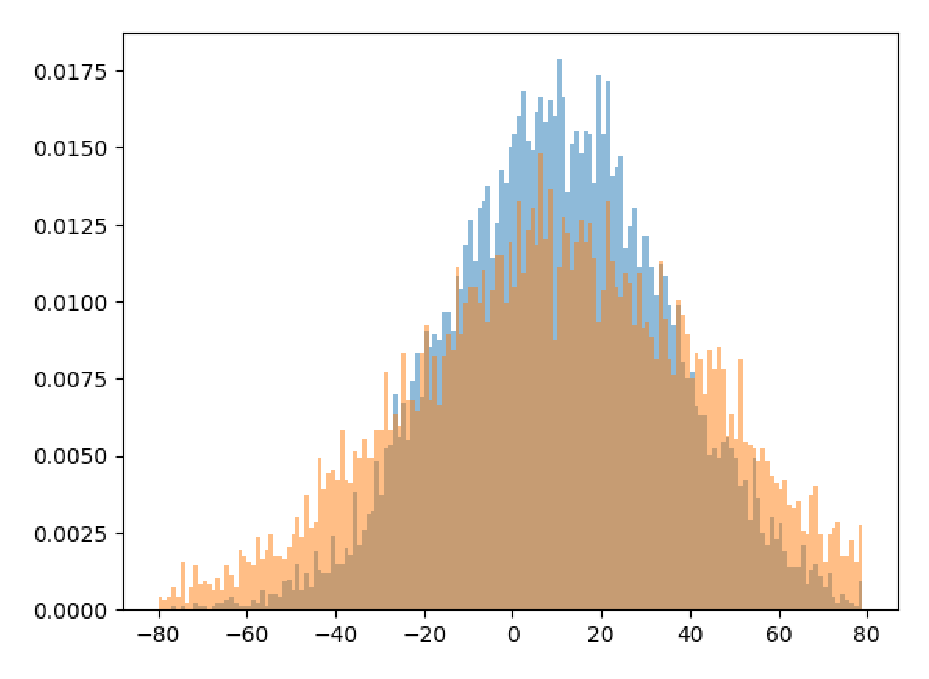
\includegraphics[scale=0.6]{colado4}
\par\end{center}

A seguir, impusemos uma restrição segundo a qual cada agente só pode contrair um empréstimo se não tiver uma dívidas em aberto (isto é, a máxima dívida possível é de uma moeda). Podemos observar que o sistema atinge um equilíbrio com um limite inferior em -1.
\begin{center}
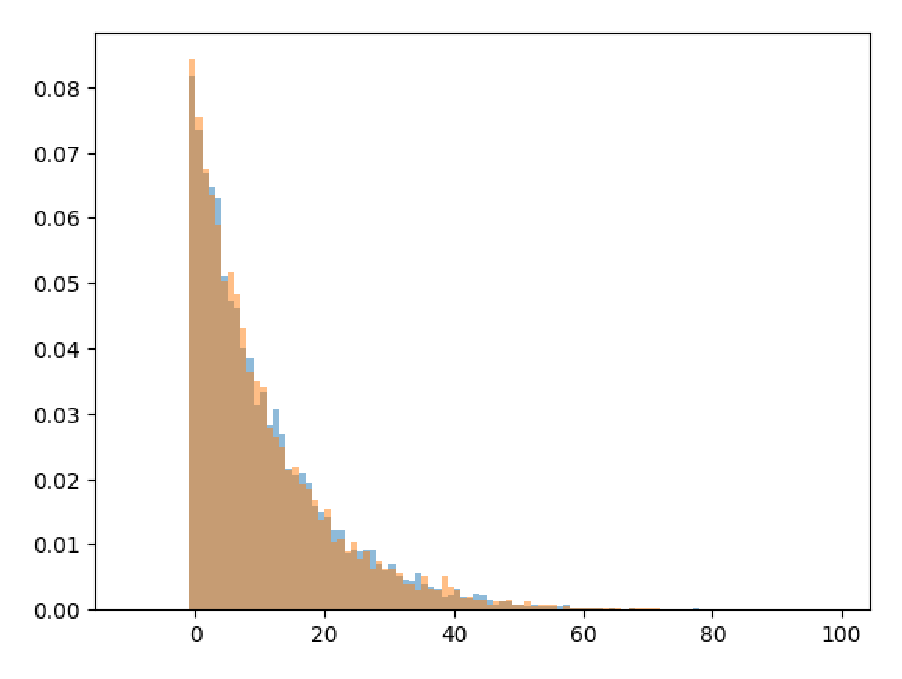
\includegraphics[scale=0.6]{colado5}
\par\end{center}

\textbf{Falácia 9}: As taxas de juros estabilizam a dívida.

Esta é uma falácia semelhante, a verdade é que as taxas de juros, na realidade, tornam o sistema ainda mais instável. Como mencionado anteriormente, apenas as restrições à dívida são capazes de estabilizar o sistema.

Abaixo, temos duas situações muito semelhantes ao caso anterior, mas agora com uma taxa de juros de 100\%. Ou seja, quando um agente toma um empréstimo de uma moeda, ele contrai uma dívida de duas moedas. Como discutido, podemos ver que o sistema se torna ainda mais instável, levando claramente a uma separação da sociedade em dois grupos: aqueles com riqueza positiva e aqueles com riqueza negativa. Assim como no caso sem juros, não há ponto de equilíbrio para o sistema.
\begin{center}
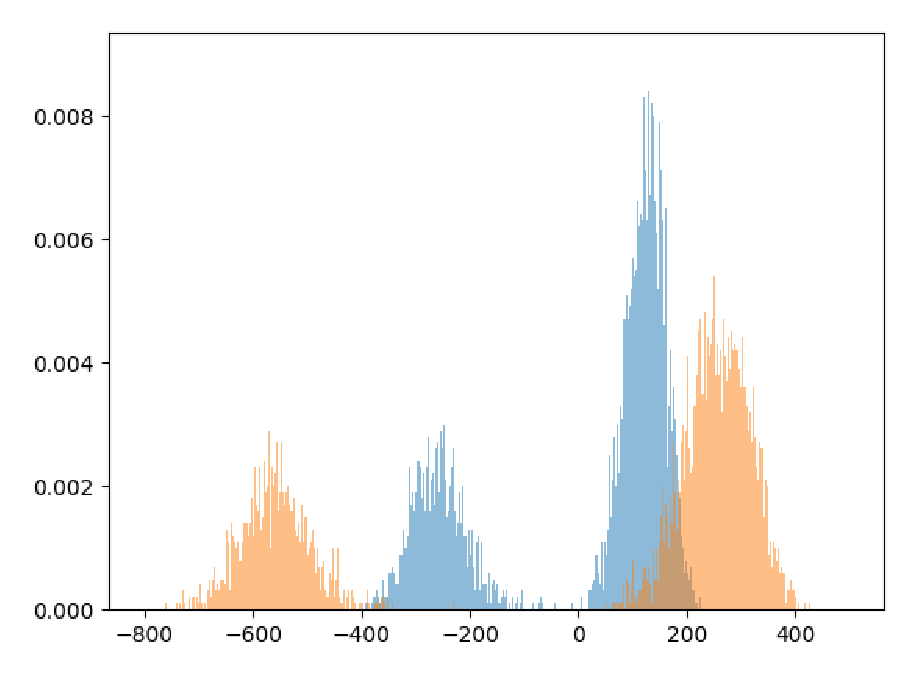
\includegraphics[scale=0.6]{colado6}
\par\end{center}

Ao adicionarmos novamente a restrição de que um agente não pode contrair um novo empréstimo enquanto ainda estiver endividado, criamos um limite inferior e permitimos mais uma vez que o sistema atinja o equilíbrio.
\begin{center}
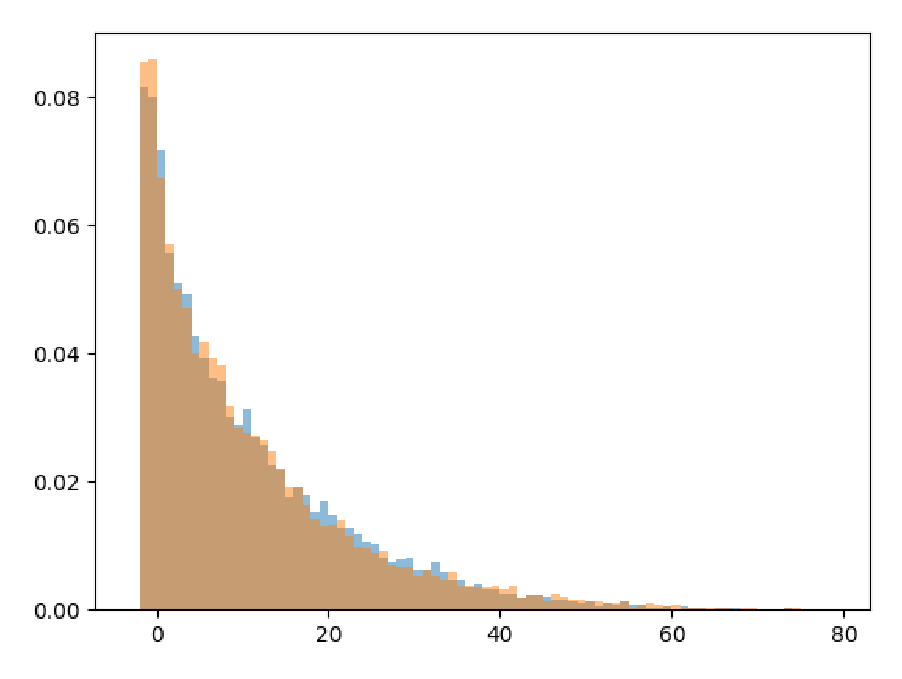
\includegraphics[scale=0.6]{colado7}
\par\end{center}

\textbf{Falácia 10}: Modelos econômicos em que as dívidas são sempre pagas conforme prometido. Por um lado, se este for realmente o caso, podemos simplesmente omitir o mecanismo de dívida, como é implicitamente assumido em muitos modelos. No entanto, é provável que alguns agentes não serão capazes de pagar suas dívidas, uma vez que esse processo parece ser irreversível. Um possível resultado é que o agente declare falência, anulando assim a nota promissória entre as partes.

Outra possibilidade é que o agente contraia novas dívidas para quitar as antigas. Essa opção adia o prazo de pagamento, mas a dívida total no sistema continuará a crescer até atingir um valor crítico, desencadeando uma cascata massiva de falências.

O crescimento do crédito e seu colapso são processos que ocorrem de forma altamente correlacionada e sincronizada. A compreensão conceitual e a descrição matemática da transição entre a expansão e a contração da dívida permanecem problemas em aberto na econofísica.

\textbf{Falácia 11}: Os bancos criam dinheiro.

Na realidade, eles criam dívida. Em um nível mais abstrato, os empréstimos podem ser agregados e anonimizados pelos bancos. Os agentes que desejam emprestar dinheiro depositam dinheiro no banco, e o banco, por sua vez, empresta dinheiro a outros agentes.

Além disso, diferentemente dos empréstimos entre indivíduos, os depositantes ainda podem usar seu dinheiro. O banco cria contas correntes para os depositantes para que eles possam emitir cheques em vez de usar dinheiro em espécie, enquanto o dinheiro depositado é colocado pelo banco comercial como reservas no banco central. Assim, o banco tem duas faces: uma voltada para os consumidores (com depósitos e empréstimos) e outra voltada para o banco central, onde ocorrem as transações entre bancos quando os cheques são compensados.

Quando o agente 1, que tem uma conta no banco A, emite um cheque de transferência para o agente 2, que tem uma conta no banco B, um valor correspondente de reservas é transferido do banco A para o banco B no banco central. Portanto, as transações interbancárias representam mais uma camada da economia monetária acima das transações individuais. O princípio da conservação monetária aplica-se às reservas bancárias, que são meramente transferidas entre bancos.

Os bancos processam um volume de transferências muito maior do que o volume de suas reservas. Se o agente 1 transfere dinheiro para o agente 2 e ambos possuem contas no mesmo banco, não há transferência de reservas entre os bancos, apenas uma alteração nos saldos digitais de suas contas. Além disso, muitos clientes dos bancos A e B realizam transações em ambas as direções, de modo que esses fluxos se anulam e a transferência líquida diária de reservas é muito menor do que o volume total de transações. Por fim, os bancos também podem contrair empréstimos temporários de outros bancos ou do banco central, portanto, a discussão sobre empréstimos individuais se repete no nível dos próprios bancos.

No entanto, quando o agente 1 deposita dinheiro no banco, ele acredita que ainda possui esse dinheiro. E quando o agente 2 contrai um empréstimo do banco, ele também acredita que agora possui dinheiro. É isso que dá a impressão de que a quantidade total de dinheiro no sistema dobrou. Contudo, o aumento do dinheiro em circulação entre os agentes é exatamente igual ao aumento da dívida no sistema. Tomar um empréstimo não é o mesmo que receber dinheiro como pagamento, o agente que toma o empréstimo permanece conectado ao banco. Outra forma de ver isso é que a criação de dívida pelos bancos não altera as reservas dos bancos no banco central, que permanecem sujeitas à lei da conservação. Assim, essa chamada criação de moeda endógena por meio da dívida difere fundamentalmente da criação de moeda exógena que ocorre quando o Estado injeta dinheiro no sistema.

\textbf{Falácia 12}: A exigência de reserva limita o endividamento máximo.

Vamos agora perguntar quanto “dinheiro” os bancos podem criar dessa forma.

Por regulamentação, os bancos são obrigados a manter reservas equivalentes a uma fração $R$ de todos os depósitos. Se tivermos um montante inicial total de dinheiro $M_{0}$ depositado nos bancos, o montante disponível para empréstimos é $(1-R)M_{0}$. Se esse montante for depositado novamente, a quantidade disponível para um novo empréstimo passa a ser $(1-R)^{2}M_{0}$. Ou seja, na primeira rodada tínhamos $(1-R)M_{0}$ disponível para empréstimos, na segunda rodada $(1-R)^{2}M_{0}$ e na n-ésima rodada teremos $(1-R)^{n}M_{0}$. Somando tudo isso, o montante total de dinheiro disponível para empréstimos é:

\[
\sum^{\infty}_{n=1}(1-R)^{n}M_{0}
\]

Se incluirmos o depósito inicial, $M_{0}$ será:

\[
M=\sum^{\infty}_{n=0}(1-R)^{n}M_{0}
\]

Podemos reescrever como:

\[
\frac{M}{M_{0}}=\sum^{\infty}_{n=0}(1-R)^{n}
\]

Uma série geométrica é definida como:
\[
\sum^{\infty}_{n=0}ar^{n}
\]

Se $|r|<1$, a série converge no limite para $\frac{a}{1-r}$. Aqui $a=1$ e $|r|$ = $|1-R|<1$ , então a soma tende a:

\[
\frac{M}{M_{0}}=\frac{1}{1-(1-R)}=\frac{1}{R}
\]

Se o dinheiro $M_{0}$ for o depósito inicial, o montante gerado por empréstimos será $M-M_{0}$. Portanto:

\[
\frac{M-M_{0}}{M_{0}}=\frac{M}{M_{0}}-1=\frac{1}{R}-1=\frac{1-R}{R}
\]

Isso significa que, para um depósito inicial de $M_{0}$, será gerado um novo montante igual a $M_{0}(\frac{1-R}{R})$. Além da exigência de reservas, os bancos também mantém uma reserva adicional para liquidar transações interbancárias.

No entanto, esses limites são flexíveis, não rígidos. Por exemplo, nos Estados Unidos, a exigência de reservas se aplica apenas a certas instituições financeiras e apenas a certos tipos de contas; existem até países sem qualquer exigência de reservas. Portanto, essa restrição é mais um mito do que um fato. Na prática, os bancos podem criar dívidas sem limite.

É evidente, porém, que se as pessoas pudessem tomar empréstimos sem restrições, pagariam por bens e serviços inteiramente com dinheiro emprestado. Se os bancos pudessem " criar dinheiro"{} facilmente, eles o criariam para si mesmos. Mesmo assim, ainda existe a necessidade de que as dívidas sejam pagas quando vencem, semelhante ao que discutimos anteriormente em relação às crises de crédito, mas em uma escala muito maior devido à agregação, consolidação, alavancagem e multiplicação pelos bancos.

Crises como a de 2008 ameaçam toda a economia, não deixando ao banco central outra opção senão intervir e salvar o sistema financeiro absorvendo as perdas. O processo ocorre em duas etapas. Primeiro, o sistema financeiro concede empréstimos enormes a tomadores que não conseguem pagar. Na segunda etapa, alguns anos depois, quando os empréstimos vencem, fica claro que esses tomadores não têm capacidade para pagar o dinheiro que tomaram emprestado.

Isso desencadeia uma grande crise que força uma autoridade monetária pública a intervir. Nos EUA, o Federal Reserve compra maciçamente esses ativos bancários, adicionando trilhões de dólares novos às reservas bancárias. Como resultado, os bancos trocam um ativo por dinheiro real criado exogenamente.

Assim, a criação de uma crise em larga escala é parte essencial do modus operandi do sistema financeiro atual. A crise serve para transformar a dívida criada endogenamente em dinheiro real criado exogenamente.

Se o banco central pode criar dinheiro novo, a questão central passa a ser: quem receberá esse dinheiro? O banco central só pode interagir com bancos comerciais; portanto, o dinheiro inevitavelmente flui para os bancos, banqueiros e a classe alta, aumentando a desigualdade na sociedade.

\subsubsection{A fonte última do lucro monetário capitalista é o dinheiro estatal}

Esse ciclo de empréstimos, crises e resgates oferece uma visão sobre duas questões relacionadas:
\begin{enumerate}
\item Todos esperam que seu dinheiro cresça devido aos juros, mas de onde vem esse dinheiro extra se o dinheiro é conservado?
\item Em relação ao lucro capitalista, no circuito $M-C-M'$, conforme exposto por Karl Marx em O Capital.
\end{enumerate}
Suponha que os capitalistas tenham um estoque de dinheiro $M$. Eles então gastam esse dinheiro para construir fábricas, contratar trabalhadores e comprar materiais, produzindo, eventualmente, a mercadoria $C$. Seu objetivo é vender as mercadorias no mercado e terminar com um saldo $M'>M$, ou seja, um lucro.

Mas quem comprará essas mercadorias? Supondo que sejam bens de consumo para as massas, serão compradas pelos trabalhadores, que só podem pagar por elas com o dinheiro recebido dos capitalistas. Assim, no agregado, o saldo monetário líquido $M'$ dos capitalistas após a venda das mercadorias não pode exceder o saldo inicial $M$. Capitalistas individuais podem obter lucros criando prejuízos para concorrentes menos competentes, mas a classe como um todo não pode ter lucro líquido.

Juros e lucros podem ser sustentados temporariamente se os consumidores se endividarem. No entanto, em algum momento, a dívida precisa ser paga. O sistema financeiro pode usar vários artifícios para adiar o pagamento, mas eventualmente ele precisa ser quitado, e o atraso alimenta a crise. Nesse ponto, quando uma crise catastrófica explode, o Estado (o governo e o banco central) intervém e injeta dinheiro exógeno no sistema, gerando lucro e juros. Portanto, concluímos que a fonte última do lucro monetário capitalista é o dinheiro estatal.

\bibliographystyle{plain}
\bibliography{tese,Artigo1/references,Artigo2/referencias}

\end{document}
